\documentclass{ximera}

\input{../../../preamble.tex}


\definecolor{fvdnavy}{HTML}{071D43}
\definecolor{fvdcyan}{HTML}{20BFC6}
\definecolor{fvdcyanlight}{HTML}{EFFCFB}
\definecolor{fvdmagenta}{HTML}{F10D69}
\definecolor{fvdmagentalight}{HTML}{FFF1F7}
\definecolor{fvdtext}{HTML}{163044}





%=================================================
% Pedagogische omgevingen
% PDF: tcolorbox
% HTML: learning-box
%=================================================

\newenvironment{voorkennis}
{%
    \ifdefined\HCode
        \HCode{%
<section class="learning-box learning-box--prior">
<div class="learning-box__header">
<span class="learning-box__icon" aria-hidden="true"></span>
<span class="learning-box__title">Voorkennis</span>
</div>
<div class="learning-box__content">
        }%
        \begin{itemize}
    \else
       \begin{tcolorbox}[
    enhanced,
    breakable,
    colback=fvdcyanlight,
    colframe=fvdcyan,
    coltext=fvdtext,
    boxrule=0.5pt,
    leftrule=4pt,
    arc=4mm,
    outer arc=4mm,
    left=7mm,
    right=6mm,
    top=5mm,
    bottom=5mm,
    before skip=6mm,
    after skip=6mm,
    title=Voorkennis,
    coltitle=fvdcyan,
    fonttitle=\bfseries\Large,
    attach title to upper={\par\smallskip},
    boxed title style={
        empty,
        left=0mm,
        right=0mm,
        top=0mm,
        bottom=0mm
    },
    overlay={
        \draw[
            fvdcyan,
            line width=0.5pt
        ]
        ([xshift=42mm,yshift=-13mm]frame.north west)
        --
        ([xshift=-7mm,yshift=-13mm]frame.north east);
    }
]
        \begin{itemize}
    \fi
}
{%
    \end{itemize}
    \ifdefined\HCode
        \HCode{%
</div>
</section>
        }%
    \else
        \end{tcolorbox}
    \fi
}


\newenvironment{leerdoelen}
{%
    \ifdefined\HCode
        \HCode{%
<section class="learning-box learning-box--goals">
<div class="learning-box__header">
<span class="learning-box__icon" aria-hidden="true"></span>
<span class="learning-box__title">Leerdoelen</span>
</div>
<div class="learning-box__content">
        }%
        \begin{itemize}
    \else
\begin{tcolorbox}[
    enhanced,
    breakable,
    colback=fvdmagentalight,
    colframe=fvdmagenta,
    coltext=fvdtext,
    boxrule=0.5pt,
    leftrule=4pt,
    arc=4mm,
    outer arc=4mm,
    left=7mm,
    right=6mm,
    top=5mm,
    bottom=5mm,
    before skip=6mm,
    after skip=6mm,
    title=Leerdoelen,
    coltitle=fvdmagenta,
    fonttitle=\bfseries\Large,
    attach title to upper={\par\smallskip},
    boxed title style={
        empty,
        left=0mm,
        right=0mm,
        top=0mm,
        bottom=0mm
    },
    overlay={
        \draw[
            fvdmagenta,
            line width=0.5pt
        ]
        ([xshift=42mm,yshift=-13mm]frame.north west)
        --
        ([xshift=-7mm,yshift=-13mm]frame.north east);
    }
]
        \begin{itemize}
    \fi
}
{%
    \end{itemize}
    \ifdefined\HCode
        \HCode{%
</div>
</section>
        }%
    \else
        \end{tcolorbox}
    \fi
}


\addPrintStyle{../../..}

\title{Oefeningen — Domein, bereik, beelden en originelen}
\author{Ingmar Herreman}

\begin{document}

% FVD_CHAPTER_DATA_START
% Automatisch gegenereerd uit index.tex.
% Niet handmatig aanpassen.
\fvdchapterdata{4}{Van relatie naar functie}{2}
% FVD_CHAPTER_DATA_END





\maketitle
\FVDbeginExercises



\begin{oefening}[Domein en bereik uit een grafiek]{\oefB\ESS}

Beschouw de grafiek.

\begin{center}
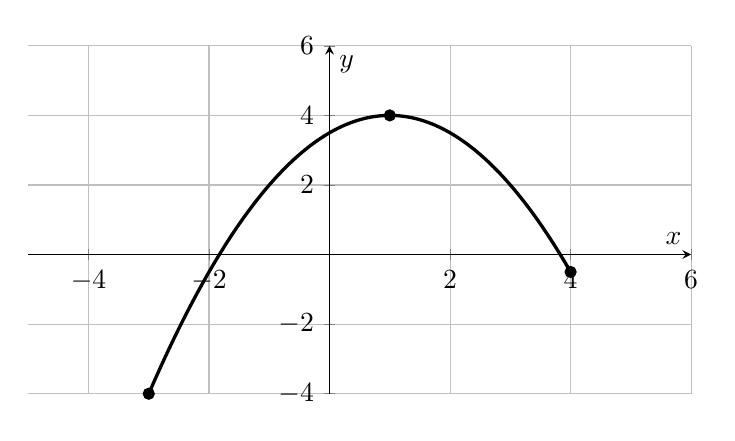
\begin{tikzpicture}
\begin{axis}[
width=10cm,height=6cm,
xmin=-5,xmax=6,ymin=-4,ymax=6,
xlabel={$x$},ylabel={$y$},
axis lines=middle,grid=both,samples=160]
\addplot[very thick,domain=-3:4] {-0.5*(x-1)^2+4};
\addplot[only marks,mark=*] coordinates {(-3,-4)(4,-0.5)(1,4)};
\end{axis}
\end{tikzpicture}
\end{center}

\begin{question}
Bepaal het domein.

\begin{oplossing}
\[
\operatorname{dom}f=[-3,4].
\]
\end{oplossing}
\end{question}

\begin{question}
Bepaal het bereik.

\begin{oplossing}
De kleinste functiewaarde is \(-4\) en de grootste \(4\). Alle waarden
daartussen worden bereikt:
\[
\operatorname{ber}f=[-4,4].
\]
\end{oplossing}
\end{question}

\end{oefening}

\begin{oefening}[Domein uit een voorschrift]{\oefB\ESS}

Bepaal telkens het domein en verantwoord de uitgesloten waarden.

\begin{question}
\[
f(x)=3x^2-2x+7.
\]
\begin{oplossing}
Een veelterm is voor elke reële \(x\) gedefinieerd:
\[
\operatorname{dom}f=\mathbb{R}.
\]
\end{oplossing}
\end{question}

\begin{question}
\[
g(x)=\frac{2x-1}{x+4}.
\]
\begin{oplossing}
\[
x+4\neq0\Longrightarrow x\neq-4,
\]
dus
\[
\operatorname{dom}g=\mathbb{R}\setminus\{-4\}.
\]
\end{oplossing}
\end{question}

\begin{question}
\[
h(x)=\sqrt{x-5}.
\]
\begin{oplossing}
\[
x-5\geq0\Longrightarrow x\geq5,
\]
dus
\[
\operatorname{dom}h=[5,+\infty[.
\]
\end{oplossing}
\end{question}

\begin{question}
\[
p(x)=\frac{1}{x^2-9}.
\]
\begin{oplossing}
\[
x^2-9\neq0\Longrightarrow x\neq-3\ \text{en}\ x\neq3.
\]
Dus
\[
\operatorname{dom}p=\mathbb{R}\setminus\{-3,3\}.
\]
\end{oplossing}
\end{question}

\end{oefening}

\begin{oefening}[Beelden]{\oefB\ESS}

Gegeven
\[
f(x)=x^2-4x+1.
\]

\begin{question}
Bereken \(f(0)\), \(f(2)\) en \(f(-1)\).

\begin{oplossing}
\[
f(0)=1,\qquad f(2)=-3,\qquad f(-1)=6.
\]
\end{oplossing}
\end{question}

\begin{question}
Welke punten op de grafiek volgen onmiddellijk uit je antwoorden?

\begin{oplossing}
\[
(0,1),\qquad(2,-3),\qquad(-1,6).
\]
\end{oplossing}
\end{question}

\end{oefening}

\begin{oefening}[Originelen]{\oefB\ESS}

Gegeven
\[
f(x)=x^2-1.
\]

\begin{question}
Bepaal de originelen van \(8\).

\begin{oplossing}
\[
x^2-1=8
\Longleftrightarrow x^2=9
\Longleftrightarrow x=\pm3.
\]
Dus \(8\) heeft de originelen \(-3\) en \(3\).
\end{oplossing}
\end{question}

\begin{question}
Bepaal de originelen van \(-1\).

\begin{oplossing}
\[
x^2-1=-1\Longleftrightarrow x^2=0\Longleftrightarrow x=0.
\]
Er is één origineel: \(0\).
\end{oplossing}
\end{question}

\begin{question}
Bepaal de originelen van \(-2\).

\begin{oplossing}
\[
x^2-1=-2\Longleftrightarrow x^2=-1.
\]
Er zijn geen reële oplossingen, dus \(-2\) heeft geen reëel origineel.
\end{oplossing}
\end{question}

\end{oefening}

\begin{oefening}[Wiskundig en praktisch domein]{\oefB\ESS}

Een voorwerp wordt vanop \(1{,}2\) m hoogte omhoog geworpen. De hoogte wordt
gemodelleerd door
\[
h(t)=1{,}2+7t-4{,}905t^2.
\]

\begin{question}
Wat is het wiskundige domein van het veeltermvoorschrift?

\begin{oplossing}
\[
\mathbb{R}.
\]
\end{oplossing}
\end{question}

\begin{question}
Waarom is dit niet het realistische domein van het model?

\begin{oplossing}
\(t\) is de verstreken tijd sinds het werpen. Negatieve tijden horen niet bij
de beschreven beweging. Bovendien stopt het eenvoudige vluchtmodel zodra
de bal de grond bereikt.
\end{oplossing}
\end{question}

\begin{question}
Gebruik GeoGebra om te schatten wanneer de bal de grond raakt en geef daarmee
een realistisch tijdsinterval.

\begin{oplossing}
De positieve oplossing van \(h(t)=0\) is ongeveer \(t=1{,}58\) s.
Een realistisch domein is dus ongeveer
\[
[0,1{,}58].
\]
\end{oplossing}
\end{question}

\end{oefening}



\begin{oefening}[Grafiek lezen in twee richtingen]{\oefU\ESS}

Beschouw
\[
f(x)=(x-1)^2-4
\qquad\text{voor}\qquad -2\leq x\leq4.
\]

\begin{center}
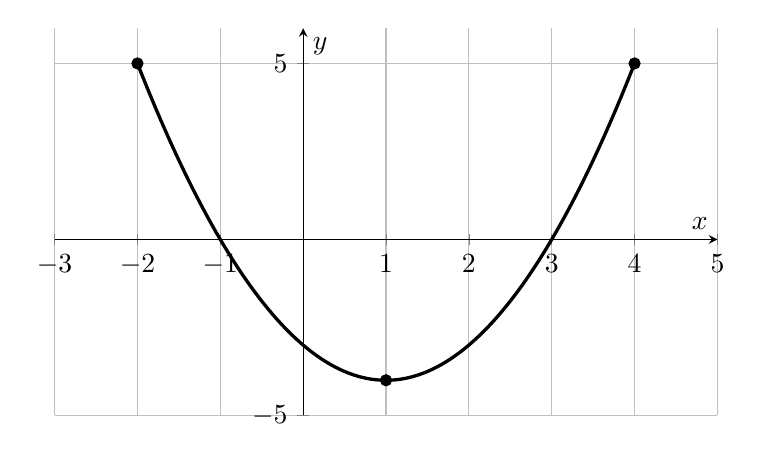
\begin{tikzpicture}
\begin{axis}[
width=10cm,height=6.5cm,
xmin=-3,xmax=5,ymin=-5,ymax=6,
xlabel={$x$},ylabel={$y$},
axis lines=middle,grid=both,samples=160]
\addplot[very thick,domain=-2:4] {(x-1)^2-4};
\addplot[only marks,mark=*] coordinates {(-2,5)(1,-4)(4,5)};
\end{axis}
\end{tikzpicture}
\end{center}

\begin{question}
Bepaal domein en bereik.

\begin{oplossing}
\[
\operatorname{dom}f=[-2,4],
\qquad
\operatorname{ber}f=[-4,5].
\]
\end{oplossing}
\end{question}

\begin{question}
Bepaal het beeld van \(3\).

\begin{oplossing}
\[
f(3)=0.
\]
\end{oplossing}
\end{question}

\begin{question}
Bepaal alle originelen van \(0\).

\begin{oplossing}
\[
(x-1)^2-4=0
\Longleftrightarrow
(x-1)^2=4
\Longleftrightarrow
x=-1\ \text{of}\ x=3.
\]
Beide waarden behoren tot het domein.
\end{oplossing}
\end{question}

\begin{question}
Heeft \(6\) een origineel? Verklaar zowel grafisch als met het bereik.

\begin{oplossing}
Nee. De horizontale lijn \(y=6\) snijdt de grafiek niet en
\[
6\notin[-4,5]=\operatorname{ber}f.
\]
\end{oplossing}
\end{question}

\end{oefening}

\begin{oefening}[GeoGebra: hoeveel originelen?]{\oefU\ESS}

Teken in GeoGebra
\[
f(x)=x^2-4x+1
\]
en maak een schuifknop \(b\). Teken vervolgens de horizontale lijn \(y=b\).

\begin{question}
Voor welke waarden van \(b\) heeft \(b\) geen origineel, precies één origineel
of twee originelen?

\begin{oplossing}
De top ligt in
\[
(2,-3).
\]
Daarom:
\[
b<-3:\ \text{geen origineel},
\]
\[
b=-3:\ \text{één origineel},
\]
\[
b>-3:\ \text{twee originelen}.
\]
\end{oplossing}
\end{question}

\begin{question}
Wat is het bereik van \(f\)?

\begin{oplossing}
\[
\operatorname{ber}f=[-3,+\infty[.
\]
\end{oplossing}
\end{question}

\begin{question}
Leg het verband uit tussen je antwoord over het aantal originelen en het bereik.

\begin{oplossing}
Een getal \(b\) behoort precies dan tot het bereik wanneer de horizontale lijn
\(y=b\) de grafiek minstens eenmaal snijdt. Het aantal snijpunten is het aantal
originelen van \(b\).
\end{oplossing}
\end{question}

\end{oefening}

\begin{oefening}[Sensor met beperkt meetbereik]{\oefU\ESS}

Een temperatuursensor wordt gebruikt tussen \(-20^\circ\mathrm C\) en
\(80^\circ\mathrm C\). In dat bereik wordt de uitgangsspanning gemodelleerd door
\[
U(T)=0{,}50+0{,}020T,
\]
met \(U\) in volt.

\begin{question}
Geef het praktische domein.

\begin{oplossing}
\[
[-20,80].
\]
\end{oplossing}
\end{question}

\begin{question}
Bepaal het praktische bereik.

\begin{oplossing}
\[
U(-20)=0{,}10,\qquad U(80)=2{,}10.
\]
Omdat het verband lineair stijgt:
\[
\operatorname{ber}U=[0{,}10,2{,}10].
\]
\end{oplossing}
\end{question}

\begin{question}
Wat betekent \(U(35)=1{,}20\) in deze context?

\begin{oplossing}
Bij een temperatuur van \(35^\circ\mathrm C\) voorspelt het model een
uitgangsspanning van \(1{,}20\) V.
\end{oplossing}
\end{question}

\begin{question}
Een spanning van \(1{,}50\) V wordt gemeten. Bepaal de bijbehorende temperatuur.

\begin{oplossing}
\[
0{,}50+0{,}020T=1{,}50
\Longrightarrow
T=50.
\]
De gemeten spanning komt volgens het model overeen met \(50^\circ\mathrm C\).
\end{oplossing}
\end{question}

\end{oefening}

\begin{oefening}[Codomein is niet hetzelfde als bereik]{\oefU\ESS}

Beschouw
\[
f:\mathbb{R}\to\mathbb{R}:x\mapsto x^2.
\]

\begin{question}
Geef domein, codomein en bereik.

\begin{oplossing}
\[
\operatorname{dom}f=\mathbb{R},
\qquad
\text{codomein}=\mathbb{R},
\qquad
\operatorname{ber}f=[0,+\infty[.
\]
\end{oplossing}
\end{question}

\begin{question}
Leg uit waarom \(-4\) wel tot het codomein behoort maar niet tot het bereik.

\begin{oplossing}
Het codomein is hier vooraf als \(\mathbb R\) opgegeven. Maar voor reële \(x\)
is \(x^2\geq0\), zodat geen enkele invoer het beeld \(-4\) heeft.
\end{oplossing}
\end{question}

\end{oefening}



\begin{oefening}[Ontwerp een functie met opgegeven domein en bereik]{\oefG}

Construeer een functie waarvan
\[
\operatorname{dom}f=[-3,5]
\qquad\text{en}\qquad
\operatorname{ber}f=[-2,4].
\]

Geef minstens twee wezenlijk verschillende oplossingen en teken hun grafieken.
Controleer je voorbeelden met GeoGebra.

\begin{oplossing}
Er zijn veel oplossingen. Een eenvoudig voorbeeld is de lineaire functie
die \((-3,-2)\) met \((5,4)\) verbindt:
\[
f(x)=\frac34x+\frac14,\qquad -3\leq x\leq5.
\]
Een andere oplossing kan een geschikte paraboolboog of een meervoudig
functievoorschrift zijn, zolang precies het opgegeven domein en bereik ontstaan.
\end{oplossing}

\end{oefening}

\begin{oefening}[Een fysisch model kritisch begrenzen]{\oefG}

Voor een eenvoudig model van het elektrisch vermogen geldt
\[
P(I)=15I^2.
\]

Een leerling beweert:
``Het domein is \(\mathbb R\), dus elke reële stroomsterkte is fysisch mogelijk.''

Analyseer deze uitspraak. Maak expliciet onderscheid tussen:
\begin{enumerate}
    \item het domein van het algebraïsche voorschrift;
    \item een gekozen tekenconventie voor de stroomsterkte;
    \item beperkingen van een werkelijk elektrisch systeem.
\end{enumerate}

\begin{oplossing}
Als algebraïsch voorschrift is \(15I^2\) voor elke reële \(I\) gedefinieerd.
Negatieve \(I\) kan bovendien fysisch betekenis hebben wanneer het teken de
stroomrichting aangeeft. Daaruit volgt echter niet dat elke reële waarde
praktisch mogelijk is: bron, weerstand, bedrading en meetapparatuur hebben
fysische grenzen. Het realistische domein hangt dus van de concrete opstelling af.
\end{oplossing}

\end{oefening}



\end{document}
